% Proposta: Figura 4 do Cap. I (etapas do ARIMA) só com o conceito. 15/11/2026, pedido do autor.
% Fora do TG até o autor decidir. Gerar com make.
\documentclass[11pt,a4paper]{article}
\usepackage[T1]{fontenc}
\usepackage[utf8]{inputenc}
\usepackage[brazil]{babel}
\usepackage{mathptmx}
\usepackage[margin=2.2cm]{geometry}
\usepackage{graphicx,booktabs,array,caption}
\setlength{\parskip}{4pt}
\setlength{\parindent}{0pt}
\title{Figura 4 do Capítulo I: o ARIMA como conceito}
\author{Proposta para o autor decidir}
\date{15/11/2026}
\begin{document}
\maketitle

\section*{O pedido}
A Figura 4 (etapas de aplicação do ARIMA) mostra o que o robô faz: teste ADF, grade de 0 a 4 com AIC,
Hannan-Rissanen, reseleção a cada 21 pregões. Como está no Capítulo I, que apresenta os modelos, a figura
deveria mostrar o ARIMA em geral. Os detalhes da implementação continuam no Capítulo II, na seção
``Estimação do ARIMA'', que já diz tudo isso em texto.

\section*{O que muda}
\begin{center}\small
\begin{tabular}{>{\raggedright}p{0.42\textwidth} >{\raggedright\arraybackslash}p{0.48\textwidth}}
\toprule
Figura atual & Propostas A e B \\
\midrule
Janela com o logaritmo dos preços de fechamento & Série histórica de preços \\
Teste ADF: há raiz unitária? (sim: diferenciar) & A série é estacionária? (não: diferenciar) \\
Para cada $p$ e $q$ de 0 a 4, estimar o modelo e calcular o AIC & Comparar modelos com diferentes combinações de $p$ e $q$ \\
Ficar com o ARIMA($p$,$d$,$q$) de menor AIC & Escolher a combinação que melhor equilibra ajuste e simplicidade \\
Estimar os coeficientes por Hannan-Rissanen & Estimar os pesos $\phi$ e $\theta$ que melhor se ajustam aos dados \\
Prever o retorno do pregão seguinte & Prever o próximo valor da série \\
Sinal da previsão: direção da operação & Previsão do próximo período \\
Chaves ``refeita a cada 21 pregões'' e ``a cada pregão'' & Chaves ``escolha das ordens $p$, $d$ e $q$'' e ``ajuste e previsão'' \\
\bottomrule
\end{tabular}
\end{center}

A saída ``Resíduos: real menos previsto'' fica nas duas propostas, porque é a ponte para o GARCH, que vem logo
depois no capítulo.

\textbf{A diferença entre A e B.} A é só o conceito. B acrescenta, em cinza e fora das caixas, ``em geral,
teste ADF'' e ``em geral, critério AIC''. Os dois nomes já aparecem no texto que segue a figura (o ADF e o AIC
são explicados ali com Thomaz, 2019, e Xing et al., 2024), então B liga a figura ao texto sem prender a figura
ao que o robô faz. A ``Hannan-Rissanen'' não entra em nenhuma das duas: o Capítulo I não fala dela, e ela é uma
escolha deste trabalho, apresentada no Capítulo II.

\textbf{O que mudaria no TG.} Só o arquivo \texttt{tg/figuras/fig05-fluxo-arima.tex}. A legenda (``Etapas de
aplicação do modelo ARIMA'') e o texto que chama a figura (``A aplicação do modelo segue as etapas
representadas na Figura 4'') continuam valendo. O texto depois da figura descreve as etapas na mesma ordem:
estacionariedade, diferenciação, escolha de $p$ e $q$ pelo equilíbrio entre ajuste e número de parâmetros,
previsão e resíduos.

\clearpage
\begin{figure}[p]\centering
\caption*{\textbf{Atual} (Figura 4 do TG)}
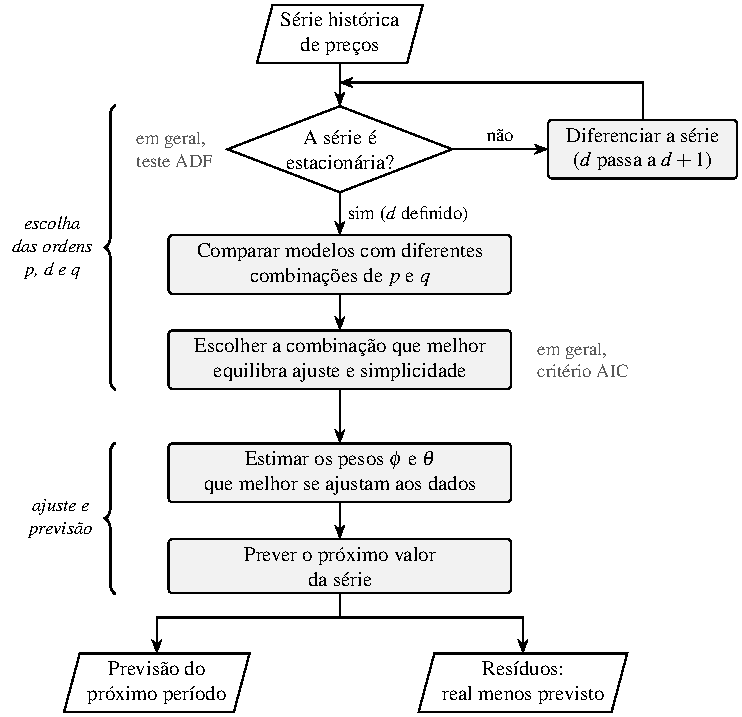
\includegraphics[width=0.78\textwidth]{../../../tg/figuras/fig05-fluxo-arima.pdf}
\end{figure}
\clearpage
\begin{figure}[p]\centering
\caption*{\textbf{Proposta A}: só o conceito}
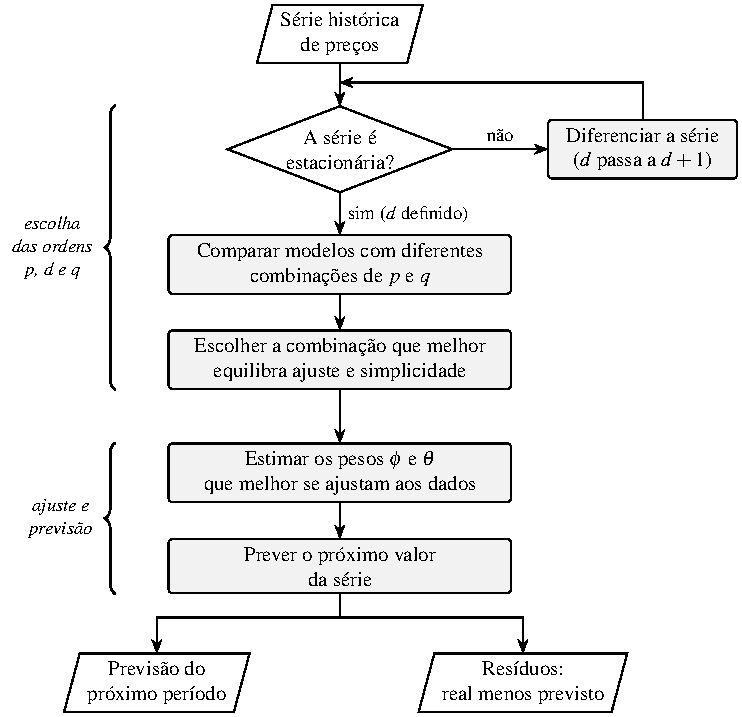
\includegraphics[width=0.78\textwidth]{fig-a.pdf}
\end{figure}
\clearpage
\begin{figure}[p]\centering
\caption*{\textbf{Proposta B}: o conceito, com a ferramenta usual de cada etapa}
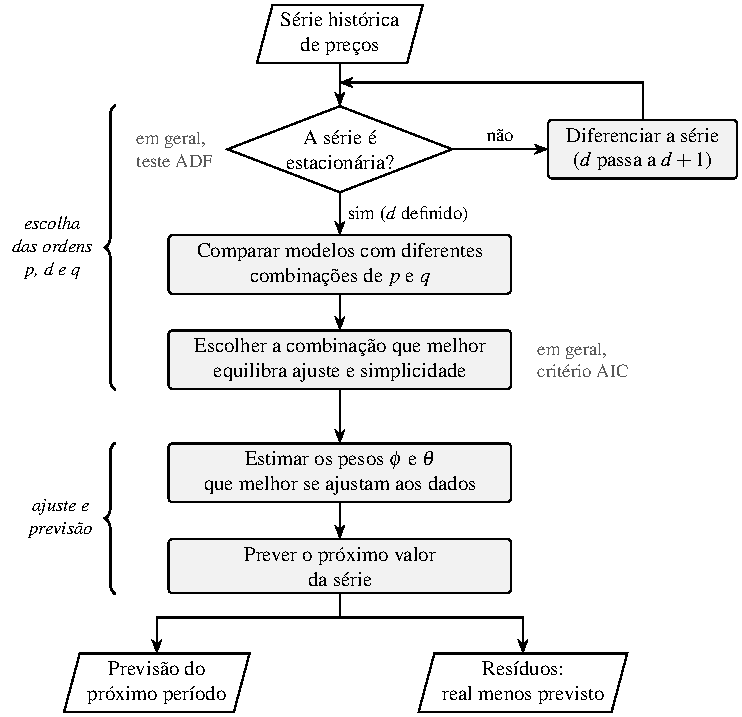
\includegraphics[width=0.78\textwidth]{fig-b.pdf}
\end{figure}
\end{document}
